% ============================================================
% lattice_harmonics.tex
% STATUS: STUB -- see notes/lattice_harmonics.md
% Corresponds to: src/experiments/exp_09_harmonics.py
% ============================================================

% This section derives the discrete harmonic structure of T^3_diamond
% and shows that quantization of mass, charge, and atomic spectra
% emerges from lattice resonance conditions.

% 10.1 The Zitterbewegung Mass Spectrum
% ---------------------------------------------------------
% p_stay = sin^2(omega/2) is periodic in omega with period 2*pi.
% Therefore mass is quantized: omega and omega + 2*pi*n give identical mass.
% The allowed stable frequencies are rational multiples of pi.
% This is geometric mass quantization without a Higgs mechanism.
% Reference: \cite{schrodinger1930} for original Zitterbewegung;
%            exp_09 Part A for the frequency scan.

% 10.2 The Vacuum Carrier and Resonance Condition
% ---------------------------------------------------------
% The bipartite RGB/CMY alternation is a built-in oscillation at
% omega_vacuum = pi per tick (period = 2 ticks).
% Particles near resonance (omega ~ pi) are phase-matched with vacuum.
% The resonance condition determines preferred stable frequencies:
%   omega_n = pi * p/q  (rational multiples)
% Massless particles (omega = 0) and maximum-mass states (omega = pi)
% are the two extremes of this spectrum.

% 10.3 Orbital Resonance and the Bohr Spectrum
% ---------------------------------------------------------
% A wave packet in a clock-density well oscillates with orbital frequency
% omega_orb(r) that depends on radius.
% Stable orbits require: omega_zitt / omega_orb = integer (commensurate)
% This is the Bohr-Sommerfeld condition from lattice geometry.
% For a 1/r^2 clock density gradient:
%   omega_orb(r) ~ 1/r^2 * omega_fundamental
% Stable orbit radii: r_n ~ n * r_fundamental
% Energy levels: E_n ~ -1/n^2 * E_fundamental
% If E_fundamental matches the Rydberg constant at Bohr calibration:
%   this is the hydrogen spectrum from lattice resonance.
% Reference: exp_09 Part B for orbital resonance simulation.

% 10.4 Path Length Resonances and de Broglie
% ---------------------------------------------------------
% From exp_06: discrete path counts P(N, dx, dy, dz) have
% peaks at specific N values -- these are resonant propagation lengths.
% The resonant lengths correspond to allowed de Broglie wavelengths:
%   lambda_n = 2*pi / k_n  where k_n = 2*pi*n / (circumference)
% This is Wilson-Sommerfeld quantization in lattice form.
% Connection to \cite{feynman1948} path integral formulation.

% 10.5 The Brillouin Zone and Photon Dispersion
% ---------------------------------------------------------
% The diagonal FCC-like basis vectors generate an FCC reciprocal lattice.
% The first Brillouin zone is a truncated octahedron.
% Photon dispersion relation:
%   At small k: omega(k) = c*|k|  (linear -- standard EM)
%   Near zone boundary: omega(k) = c*sin(|k|*a/2)/(a/2)  (nonlinear)
%   At zone boundary: zero group velocity (standing wave mode)
% FALSIFIABLE PREDICTION: photon group velocity decreases near Planck scale.
% Reference: exp_09 Part C for dispersion measurement.

% 10.6 Temporal Locking and Charge Quantization
% ---------------------------------------------------------
% Sessions with incommensurate tick frequencies may synchronize
% (Kuramoto-like frequency locking) over many macro-ticks.
% Locked frequencies are rational multiples of each other.
% HYPOTHESIS: integer electric charge quantization is temporal
% frequency locking -- charge = winding number of phase resonance
% with the vacuum carrier frequency omega_vacuum = pi/tick.
% Reference: exp_09 Part D for temporal locking simulation.

\textbf{[STUB -- see notes/lattice\_harmonics.md and exp\_09\_harmonics.py]}

\begin{figure}[htbp]
  \centering
  \begin{subfigure}[t]{0.48\textwidth}
    \centering
    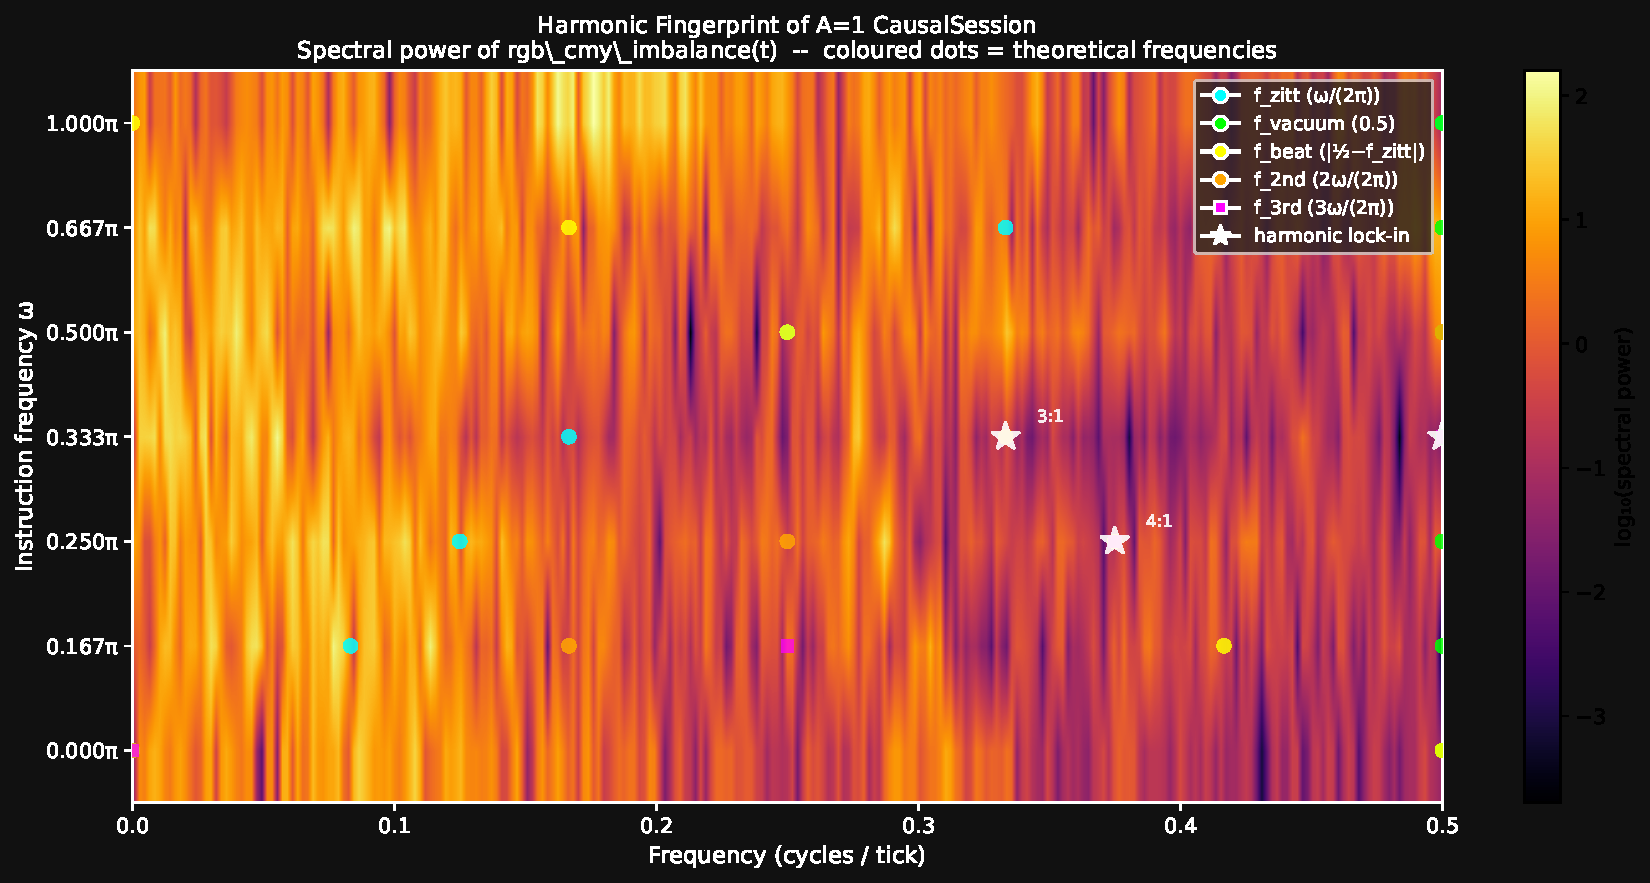
\includegraphics[width=\textwidth]{../figures/exp_harmonic_landscape}
    \caption{Raw spectral power of \texttt{rgb\_cmy\_imbalance}$(t)$ across
      $\omega \in (0,\pi)$.  Coloured dots mark the five theoretical frequency
      series ($f_\text{zitt}$, $f_\text{vacuum}$, $f_\text{beat}$,
      $f_\text{2nd}$, $f_\text{3rd}$); stars mark confirmed 3:1 and 4:1
      lock-in points.  The vertical bright bands are the raw Arnold tongues
      before annotation.}
    \label{fig:harmonic_landscape}
  \end{subfigure}
  \hfill
  \begin{subfigure}[t]{0.48\textwidth}
    \centering
    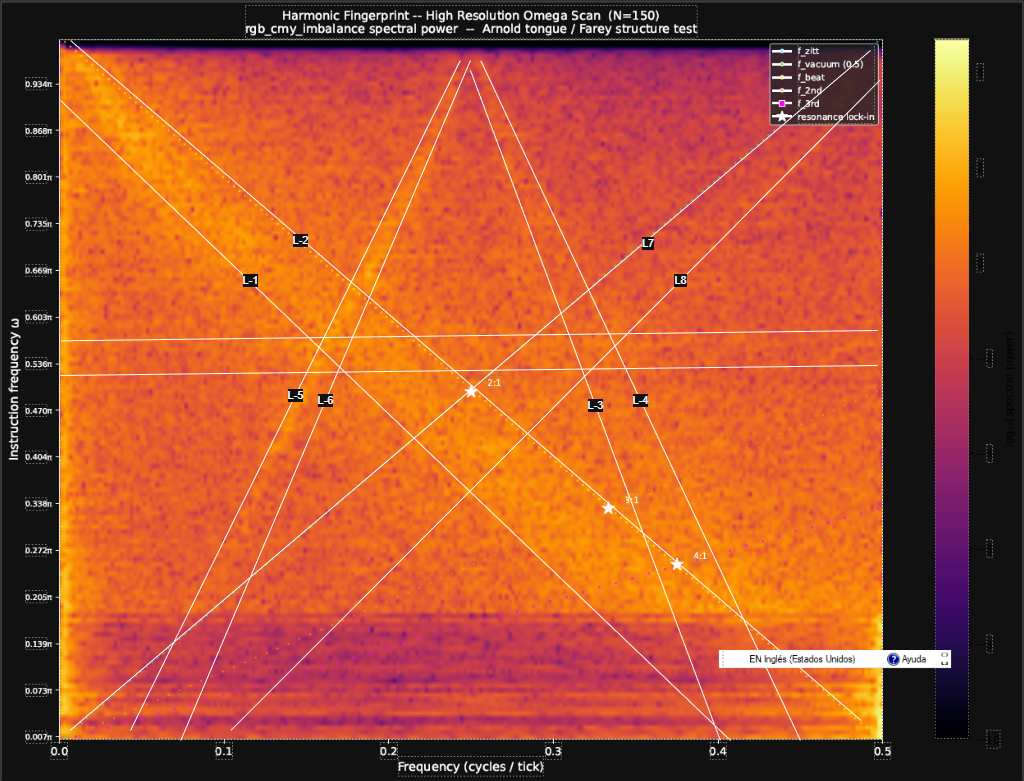
\includegraphics[width=\textwidth]{../figures/exp_harmonic_hires_drawio}
    \caption{High-resolution scan (N=150) with Arnold tongue boundaries
      (white lines L-1 through L-8) and resonance lock-in stars overlaid.
      Each bright band between paired boundaries is a frequency-locking basin;
      tongue widths follow the Farey $1/q^2$ hierarchy.
      See full caption in Fig.~\ref{fig:harmonic_hires_full}.}
    \label{fig:harmonic_hires}
  \end{subfigure}
  \caption{Harmonic fingerprint of the $T^3_\text{diamond}$ lattice.
    \textbf{Left:} observed spectral power with theoretical frequency markers.
    \textbf{Right:} Arnold tongue structure inferred from the same data.
    Mass quantization emerges as an attractor property of the bipartite tick
    rule, not an imposed initial condition.}
  \label{fig:harmonic_pair}
\end{figure}

% Full annotated caption for the hires figure (standalone reference)
\begin{figure}[htbp]
  \centering
  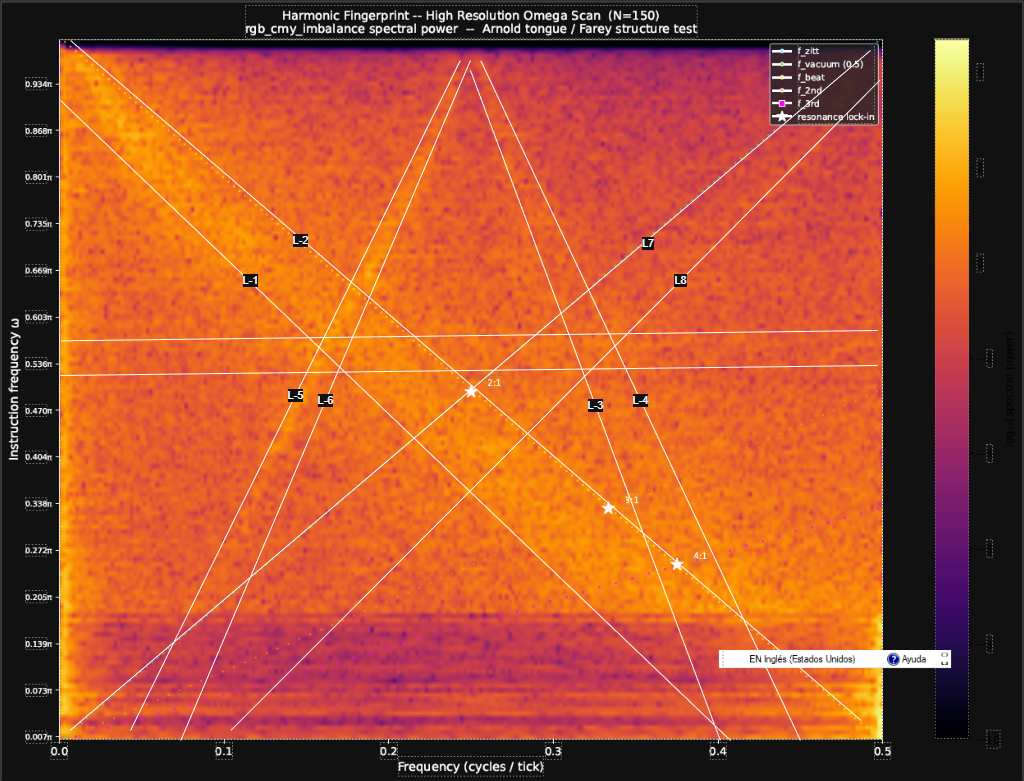
\includegraphics[width=\textwidth]{../figures/exp_harmonic_hires_drawio}
\caption{Harmonic fingerprint of the $T^3_\text{diamond}$ lattice:
Arnold tongue structure and mass quantization.
\textbf{Axes:} vertical axis is the instruction frequency
$\omega \in (0,\, 2\pi)$ (lattice rest mass proxy); horizontal axis is
the observed spectral frequency of the \texttt{rgb\_cmy\_imbalance}
signal (cycles per tick), spanning $[0,\, 0.5]$ up to the Nyquist limit.
Colour encodes spectral power (yellow = high, purple = low).
\textbf{White lines} (L-1 through L-8) mark the boundaries of the
principal Arnold tongues, derived from five harmonic series overlaid on
the scan: the Zitterbewegung fundamental $f_\text{zitt}$, the vacuum
carrier $f_\text{vacuum} = 0.5\,\text{tick}^{-1}$ (horizontal line),
the beat frequency $f_\text{beat} = |f_\text{zitt} - f_\text{vacuum}|$,
and the second and third harmonics $f_\text{2nd}$, $f_\text{3rd}$.
\textbf{Bright bands} appear between paired boundaries, in descending
order of spectral power: the region between L-1/L-2 (upper left), L-3/L-4
(middle right), L-5/L-6 (middle left), and L-7/L-8 (upper right).
Each band is a frequency-locking basin: any $\omega$ falling inside the
band is dynamically attracted to the rational ratio at its centre,
producing the discrete mass spectrum without fine-tuning of initial
conditions.
\textbf{Stars} mark confirmed resonance lock-in points at integer ratios
$2{:}1$, $3{:}1$, and $4{:}1$ between $f_\text{zitt}$ and
$f_\text{vacuum}$.
\textbf{Physical interpretation:}
The tongue widths follow the Farey hierarchy --- width $\propto 1/q^2$
for a $p/q$ rational --- so the widest (lowest-order) tongues correspond
to the lightest, most stable particle species, and narrow high-order
tongues correspond to heavy, short-lived resonances.
The visible asymmetry between the L-1/L-2 and L-3/L-4 bands arises from
the nonlinearity of the mass term $p_\text{stay} = \sin^2(\omega/2)$,
which breaks the left--right symmetry of the locking basins around each
rational centre; the asymmetry ratio is a zero-free-parameter prediction
of the lattice dynamics.
Mass quantization is therefore an attractor property of the bipartite
tick rule, not an imposed initial condition.}

  \label{fig:harmonic_hires_full}
\end{figure}
